\documentclass[conference]{IEEEtran}
\IEEEoverridecommandlockouts
% The preceding line is only needed to identify funding in the first footnote. If that is unneeded, please comment it out.
% \usepackage{cite}
% The 'cite' package and biblatex are incompatible.
\usepackage{amsmath,amssymb,amsfonts}
\usepackage{algorithm}
% \usepackage{algorithmicx}
\usepackage{algpseudocode}
\renewcommand{\algorithmicrequire}{ \textbf{Input:}}
\renewcommand{\algorithmicensure}{ \textbf{Output:}}
\usepackage{graphicx}
\usepackage{subfigure}
\usepackage{textcomp}
\usepackage{xcolor}
\usepackage{enumitem}
\usepackage{amssymb}

\usepackage{tabulary}
\usepackage{spverbatim}
% \usepackage{chinesedraft}

\usepackage[style=ieee]{biblatex}
\addbibresource{bibliography/refs.bib}
\addbibresource{bibliography/epit.bib}


\algblock{Input}{EndInput}
\algnotext{EndInput}
\algblock{Output}{EndOutput}
\algnotext{EndOutput}
\newcommand{\Desc}[2]{\State \makebox[2em][l]{#1}#2}

\def\BibTeX{{\rm B\kern-.05em{\sc i\kern-.025em b}\kern-.08em
    T\kern-.1667em\lower.7ex\hbox{E}\kern-.125emX}}

\newlist{researchquestions}{enumerate}{1}
\setlist[researchquestions]{label*=\textbf{RQ\arabic*.}}
    
\begin{document}

% I see somewhere that don't use abbr. in title
\title{Augmenting Automated Mobile UI Testing with Semantic-aware Test Input Generation: A Cost-effective Approach with LLMs}

\author{
    \IEEEauthorblockN{Rui-Fan Yang}
    \IEEEauthorblockA{\textit{Guohua Memorial Middle School}\\
        Foshan, China \\
        ly-niko@qq.com}
    \and
    \IEEEauthorblockN{Yuan-Rui Li}
    \IEEEauthorblockA{\textit{Shenzhen Experimental School}\\
        Shenzhen, China \\
        leoli@6leo6.com}
    \and
    \IEEEauthorblockN{Shu-Wei Wu}
    \IEEEauthorblockA{\textit{Shenzhen Experimental School}\\
        Shenzhen, China \\
        2183220676@qq.com}
}

\maketitle

\begin{abstract}
    % Already Polished
    UI testing for mobile applications is a critical process for identifying software defects. Crafting meaningful test cases for UI testing remains a significant challenge. As the complexity of application development increases, manually creating test cases for every conceivable scenario becomes impractical, thus elevating the importance of automated testing. Although automated testing tools are extensively utilized to swiftly generate test cases, they often fail to detect intricate issues that necessitate a sequence of logical events to uncover. Our Large Language Model (LLM)-guided approach prioritizes the generation of semantically-aware input sequences, enabling the efficient creation of practical test cases within a reasonable timeframe. We assessed our method using a collection of real-world applications and benchmarked it against commonly-used tool\cite{androidUIApplicationExerciser}, which demonstrated that our tool attained a 79.2\% increase in detected activities and a 57.6\% higher success rate per activity through the analysis of semantic information and internal feature logic.

\end{abstract}

\begin{IEEEkeywords}
    Mobile UI Testing, Large Language Model, Test Input Generation, Automated GUI Testing
\end{IEEEkeywords}

\section{Introduction}
% Polished
With the proliferation of mobile applications and their widespread use in daily life, the quality requirements for mobile applications have been greatly increased, making the search for potential bugs and security issues a focal point of research. However, due to the increasingly diverse and complex features of mobile applications, traditional manual testing methods have become inefficient and unable to meet industrial requirements, thus making automated UI testing a hot research topic. \cite{testingliteraturereview}\cite{androidUIApplicationExerciser}\cite{ngo_automated_2022}\cite{lin_route_2023}\cite{gu_practical_2019} Automated testing is designed to improve code coverage and test a more diverse set of application functions. However, existing automated tests often struggle to effectively navigate to specific pages associated with particular features for comprehensive testing due to challenges in leveraging important content such as object names provided by developers and in-app text, and their association with application logic.

To achieve the purpose of testing specific features, the method of feature-based UI testing has been proposed. This approach usually involves developers manually writing test cases to implement navigation between pages of the Application Under Test (AUT). For example, the operation sequence in the figure \ref{image-ui-element-update} implements navigation from one activity to another, thereby enabling better testing of the settings interface functions.
However, with the rapid iteration of mobile applications, the fixed operation sequences between pages are highly uncertain. For instance, changes to the application interface elements in the updated application may lead to the invalidation of the original automated test cases. Therefore, existing feature-based UI testing still requires a significant amount of human labor to write and maintain test cases.

\begin{figure}[htbp]
\centering
\subfigure[In old version, the element's resource-id is 'fab\_add\_button']{
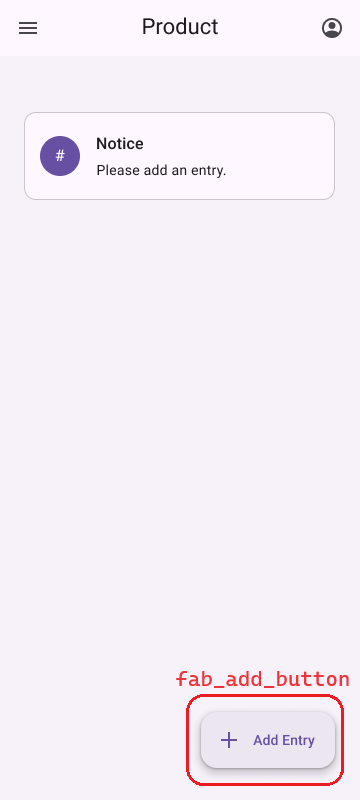
\includegraphics[scale=0.25]{assets/AppUI-FAB-labeled.png}
}
\quad
\subfigure[In new version, the element is no longer a floating action button, and the resource-id has also changed]{
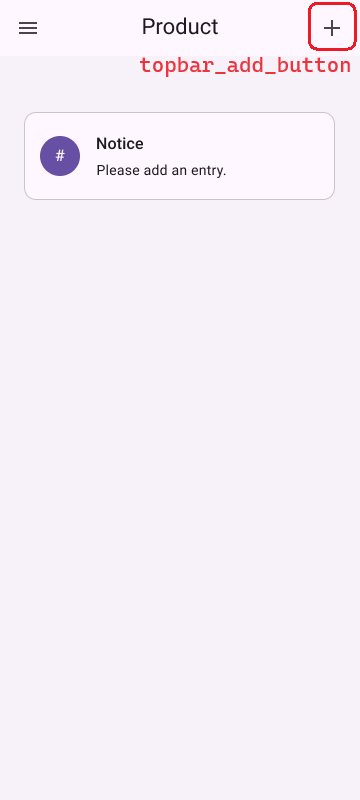
\includegraphics[scale=0.25]{assets/AppUI-TopBar-labeled.png} 
}
\caption{Different UI design cause old test script fail to work because locating the element is failed}
\label{image-ui-element-update}
\end{figure}

% Polished
The underlying issue we address stems from two primary factors:
(1) The challenge of effectively interpreting the semantic content of page text. For instance, when logging into an application, conventional tools may repeatedly fail because they do not comprehend the significance of labels such as ``username'' and ``password'' adjacent to the input fields, considering them merely generic inputs. Though these labels could be hardcoded, the vastness and variability of modern applications make it unfeasible to anticipate all text in every interface, especially with dynamically generated content like daily news.
(2) The inability to execute a coherent sequence of events. Such sequences are essential for tasks like adjusting a setting in an application's submenu, which necessitates navigating to that submenu first, then to the settings page, and eventually modifying the setting. The well-known random testing tool, Monkey, often fails at these tasks due to its random nature, making it incapable of systematically executing the required action sequences.

Despite advances in random testing and machine learning-based testing, neither approach has successfully emulated the human-like cognitive processes for recognizing user interface layouts and generating events. However, the logical structure inherent in real-world applications' activities, layouts, and especially texts, is not easily deciphered or exploited by most existing tools.

To bridge this gap, we propose our solution, a language model-based tool designed to enhance UI testing by emulating human cognitive patterns. Our tool takes the application under test (AUT), the target activity name, and an optional pre-collected path as inputs. It processes all interactive elements at each testing stage and translates them to natural language descriptions, thus integrating a language model to enrich mobile app UI testing.
Our results demonstrate that compared to traditional testing methods, the language model approach significantly boosts efficiency and success rates while more effectively revealing potential flaws, attesting to its effectiveness and superiority. This offers a new strategy for mobile app UI testing that synthesizes human-like cognitive processes.

To evaluate the effectiveness of our tool, we construct a benchmark used to evaluate the capable for finding path to deep activities, consisting of test cases from 2 highly popular industrial Android apps that are widely used in previous work \cite{dong_time-travel_2020}\cite{Wang:2018:ESA:3238147.3240465}\cite{vet-paper}\cite{toller-paper}.

In general, this paper made these contributions:
\begin{itemize}
\item Introduces a novel problem regarding automated feature-based UI testing that leverages only the targeted activity name.
\item Proposes a cost-effective methodology for automating UI testing, which entails utilizing Large Language Models (LLMs) to interpret the UI state and engender appropriate actions to navigate to specified activities.
\item Presents an evaluation showcasing the efficacy of our approach in enhancing the accesibility of UI activities by 79.2\% and achieving a 57.6\% success rate in reaching individual activities across two widely-used industrial applications.


\end{itemize}

\section{Background}
% 概括Background由哪些内容组成, Polished
The advancement of software engineering has significantly influenced mobile computing, especially concerning user interface (UI) systems. The Android platform, due to its widespread adoption, has emerged as a pivotal area for research and development, underlining the importance of an in-depth comprehension of its UI system. This section examines the fundamental concepts that underpin our research.

We begin by exploring the architecture of the Android UI system and the underlying principles that govern its operation, which are vital for app development and user engagement.

Additionally, we explore the transformative role of Large Language Models (LLMs) in UI design and testing within the Android ecosystem, shedding light on their sophisticated features that facilitate automation.

Finally, the section discusses the definitions of key terms to enhance the clarity of our discourse.

\subsection{Android UI System}
In the realm of the Android operating system, the UI framework \cite{android_layouts_in_views} is a meticulously architected hierarchy, predominantly consisting of Activities and constituent UI components. Each activity $a$ encapsulates a discrete screen outfitted with a user interface, delineated as an XML-encoded tree comprising various elements such as TextView, EditText, and Button, to name a few.

The inter-element relationships are articulated through a defined parent-child nexus, underscoring their stratified positioning within the UI schema. For example, a ViewGroup, serving as a container element, may encompass a multitude of TextView elements, signifying that these TextViews are arrayed at an equivalent hierarchical echelon.

Every individual element $w$ is endowed with an array of attributes. These attributes are instrumental in dictating user interactivity capabilities (e.g., scrollable) and in defining the visible text content. The latter is integral for the conveyance of accessibility information or for aligning with specific content identifiers within the resource ID framework.
% ===

\begin{figure}
    \centering
    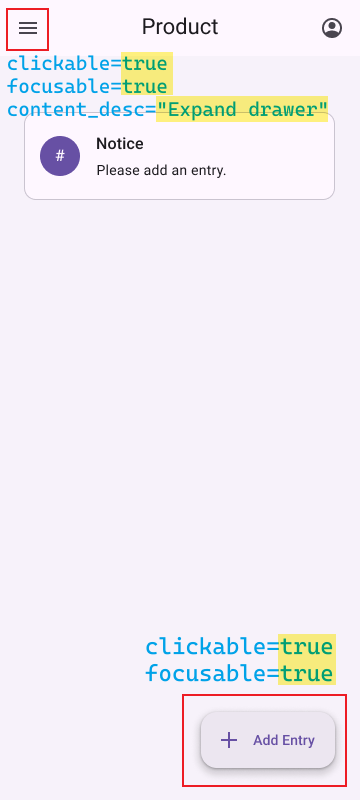
\includegraphics[width=0.5\linewidth]{assets/AppUI-FAB-attrs.png}
    \caption{This figure shows several attributes indicating whether the element can be interacted and semantic information in the attributes. Note that the ``Add Entry'' button at the right bottom corner doesn't have any semantic-meaningful attributes because of \textit{element wrapper}, which separate actionable elements and text elements apart.}
    \label{image-attrs-in-element-xml}
\end{figure}

\subsection{Large Language Model}
Large Language Models (LLMs) are advanced natural language processing tools characterized by their vast parameter space and extensive capabilities. These models employ deep learning methodologies\cite{DeepLearning} to internalize grammatical rules, semantic nuances, and contextual understanding through rigorous training on substantial data sets, supported by significant computational resources.

In recent times, LLMs have achieved remarkable progress, showcasing their versatility across a spectrum of disciplines. Among the notable instances is the ChatGPT series by OpenAI, which incorporates a Generative Pretrained Transformer (GPT)\cite{vaswani2017attention}\cite{brown2020language} architecture. Trained on exceptionally large data corpora, these models integrate methods like Reinforcement Learning from Human Feedback (RLHF)\cite{ouyang2022training} and boast hundreds of billions of parameters. As a result, they are proficient in generating coherent text, decoding and responding to inquiries, executing translation tasks, and composing summaries, among other functions.

By providing natural language prompts and steering LLMs through Prompt Engineering, we can devise potential operational sequences to assess core functionalities within software applications. To this end, we furnish the LLM with a specific testing challenge, direct it to formulate suitable input sequences, and apply these sequences to the Application Under Test (AUT). This technique permits the evaluation of various app features in a manner that closely resembles real-world user interactions.

\subsection{Android UI Testing}
Android UI Testing is designed to generate test cases derived from the application's hierarchy, thereby facilitating a more comprehensive exploration with minimal human intervention, uncovering bugs, and performing tests on the Application Under Test (AUT) with enhanced efficiency and quality. Numerous methods are available for the automated testing of mobile applications, including random testing with tools like Monkey, leveraging deep learning with artificial intelligence, and employing algorithms for more effective testing strategies. Presently, conventional testing methodologies predominantly rely on random events or manually crafted test cases, which are often inefficient and labor-intensive, yielding less than optimal outcomes.


\subsection{Definitions}    % this subsection is polished

\textbf{UI State}. Each UI state, denoted as $s$, is associated with an activity $a$ and comprises a multitude of elements. Within each state $s_1$, users can interact with specific elements such as buttons, text boxes, and scrollable containers. These interactive elements are represented as $W_{s_{1}}$.

\textbf{Command and Action}. Commands, represented as $c$, are types of UI interactions that include \textit{input}, \textit{click}, and \textit{back}, among others. The collection of all commands supported by our tool is denoted by $C_{all}$. A command $c$ is considered applicable to an element $w$ if $c \in C_w$; for instance, the \textit{input} command should only be applicable to text boxes. Actions, denoted as $e$, are described by a triplet $(w, c, v)$ where $w$ signifies the targeted element, $c$ the command executed, and $v$ any additional parameters necessary for the action (e.g. the \textit{input} command requires a textual argument representing the input text).

\textbf{Activity Path}. An activity path $p = (a_0, e_0, e_1, ..., a_1)$ traces the sequence of actions from a starting activity $a_0$ to a target activity $a_1$, through successive actions $(e_0, e_1, e_2, ...)$.

\textbf{Descriptions}. Each activity $a$ and UI state $s$ possesses a description, symbolized by $d_a$ and $d_s$ respectively, which articulates its functionality and content. The activity description $d_a$ could be provided by the developer or generated by an LLM, based on all UI states previously encountered $s_1, s_2, ...$, within the activity $a$.

% This section is polished
\section{Preliminary Study} The automated mobile application testing tool Monkey is renowned for its ability to swiftly generate a vast array of random events with designated weights, which facilitates the random invocation of application functionalities and the transition into new activities. Monkey's prevalent use in automated application testing underscores its utility. Within this section, we examine the inefficiencies inherent in Monkey's testing approach, identify their underlying causes, and underscore the imperative to integrate Large Language Models (LLMs) with the aim of refining the process of automated mobile application testing.

\subsection{Coverage of Monkey for Industrial Applications}

Our application of Monkey for automated testing on two extensively used commercial Android applications has revealed that Monkey consistently achieves only a modest activity coverage rate over prolonged test durations.

In complex industrial applications, Monkey's capacity to thoroughly probe the application's functional Activities is not satisfactory, even with considerable testing time allotted. As depicted in Table \ref{tab:monkey_cover}, Monkey achieved an average coverage of merely 42.1\% of possible Activities, which poses a considerable limitation on the testing's effectiveness and thoroughness.

\subsection{Root Cause Analysis of Activities and Edges Not Covered by Monkey}

Our analysis indicates that Monkey is hampered by its inability to execute complex scenarios which necessitate a sequential chain of input events. Additionally, it fails to reauthenticate following a log out, as exemplified by the Spotify application. These limitations have been corroborated by previous studies \cite{vet-paper}.

For instance, as illustrated in Figure \ref{fig:school-planner-sequence}, to activate the \texttt{SubjectActivity} in the School Planner application, users must navigate through a series of steps including: reaching the corresponding activity, invoking the ``Create'' button at the UI's bottom right, selecting a Subject, entering the Subject's name, saving it, and ultimately accessing the Subject. Given Monkey's propensity to execute more frequent back button presses and inadvertent area taps, it often interrupts the operational flow, thereby precluding the generation of complete test scenarios.


\begin{figure*}
    \centering
    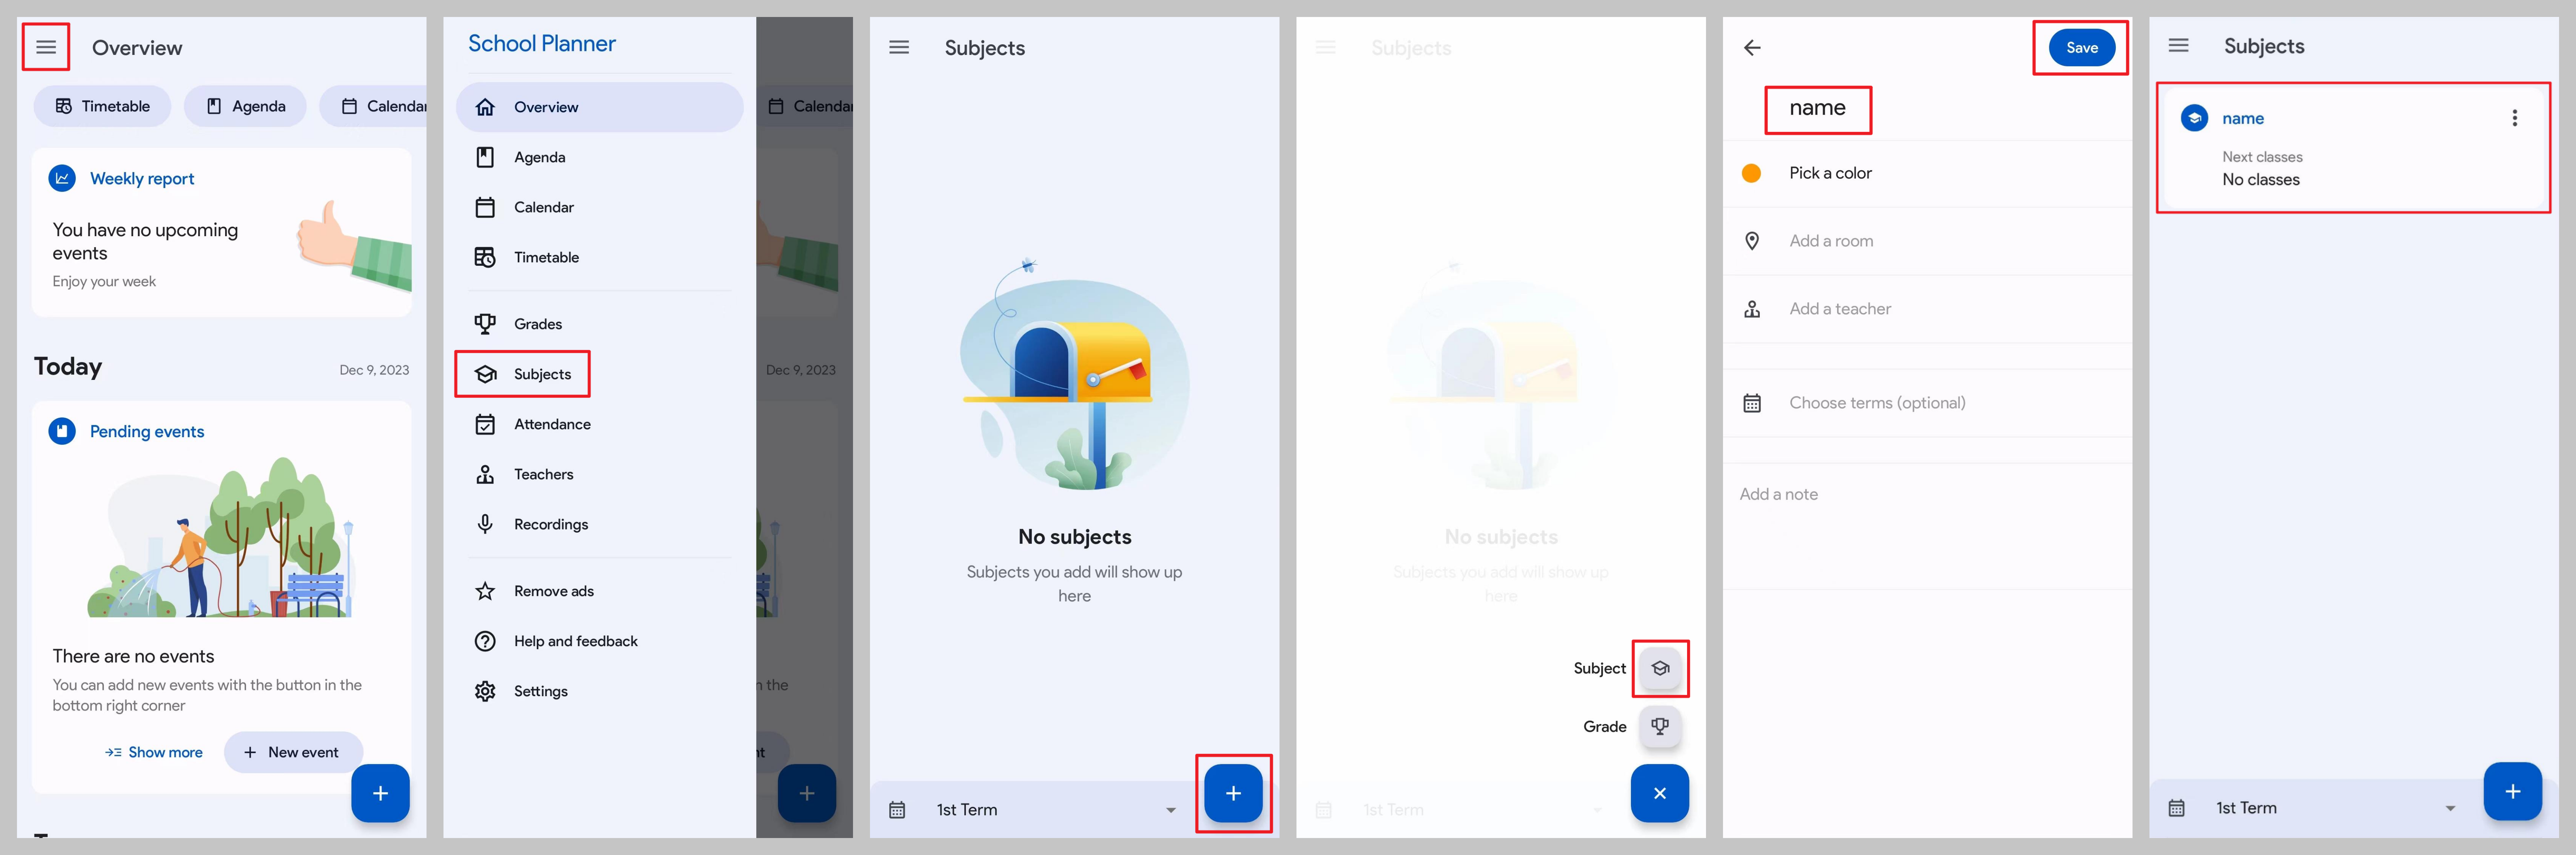
\includegraphics[width=1\linewidth]{assets/school-planner-sequence.png}
    \caption{Demonstration of achieving \textit{SubjectActivity} with a sequence of actions}
    \label{fig:school-planner-sequence}
\end{figure*}

\section{Approach}

Our methodological approach is comprised of the following steps:

\begin{enumerate}
	\item We infer the latent functionality of activities lacking explicit descriptions by analyzing their package and activity names, utilizing the Large Language Model (LLM) to generate provisional descriptions.
	\item Where accessible, we engage the LLM to pinpoint the description that most closely aligns with our target activity (for instance, to navigate to the \texttt{.settings.ThemeSettingsActivity} interface for theme configuration, one would logically initiate at the \texttt{.settings.MainActivity} settings menu), thereby grounding our exploration in relevant context.
	\item Prior to execution, we excise all textual data from the interface's hierarchical layout, submit it to the LLM to craft a concise state description reflective of the current context.
	\item We meticulously structure both target and state descriptions to integrate them into the user prompt, amalgamating this with the UI state's elemental data, and subsequently relay it to the LLM for discernment and directive. We then interpret its guidance to interact with the Application Under Test (AUT) via the execution of appropriate actions.
	\item This procedure is iteratively applied until the designated target activity is attained.
\end{enumerate}
\begin{figure*}
    \centering
    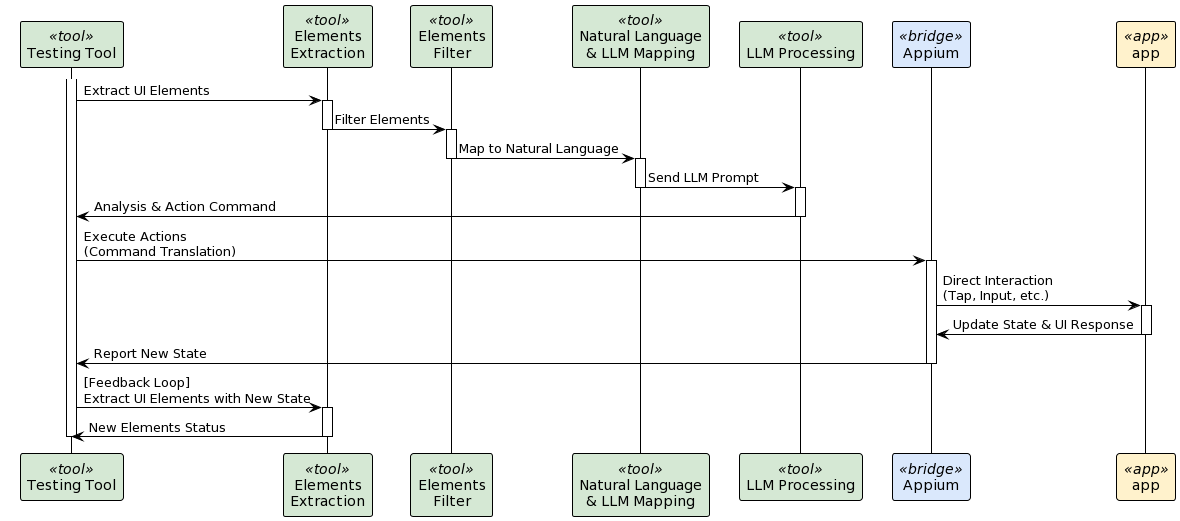
\includegraphics[width=1\linewidth]{assets/PlantUML-time-seq-graph.png}
    \caption{Architecture of our tool}
    \label{fig:enter-label}
\end{figure*}
The algorithm is delineated through the accompanying pseudocode:

\begin{algorithm}
\caption{Design Overview of Our Tool}
\label{alg_overview}
\begin{algorithmic}
    \Require{ The target activity $a_1$}
    \Ensure{ The activity path $p_{a_1}$ if success}
    \State $actions \gets []$
    \State $known\_activities \gets load\_knowledge()$
    \State $goal\_desc \gets llm\_ask(a_1)$
    \Statex $a_{start} \gets llm\_ask(goal\_description, known\_activities)$
    \State $go\_to\_best\_start\_activity(a_{start})$
    \State $start\_acivity \gets get\_current\_activity()$
    \State $start\_time \gets time()$
    % while not current_activity == target_activity:
    \While{$get\_current\_activity() \neq a_1$}
        % detect if failed due to step / time limit
        \If{$ actions.length > max\_step $}
            \State \Return $[]$
        \EndIf
        \If{$ time() - start\_time > max\_time $}
            \State \Return $[]$
        \EndIf
        % get current acivity, status
        \State $s_i \gets get\_current\_status()$
        % get current status description
        \State $d_{s_i} \gets llm\_ask(s_i)$
        % get elements
        \State $W_s \gets get\_elements(s_i)$
        % filter elements
        \State $W_s \gets filter\_elements(W_s)$
        % get elements description
        \State $elements\_descs \gets get\_descs(W_s)$
        % get elements commands
        \State $elements\_commands \gets get\_commands(W_s)$
        % pass these to LLM
        \State $llm\_input \gets [d_{s_i}, elements\_descs, $
        \Statex $\qquad \qquad elements\_commands, goal\_desc, actions]$
        \State $llm\_output \gets llm\_ask(llm\_input)$
        % extract element, command and extra
        \State $element \gets llm\_output[0]$
        \State $command \gets llm\_output[1]$
        \State $extra \gets llm\_output[2]$
        % check if valid
        \If{$is\_valid(llm\_output)$}
            % continue
            \State \textbf{continue}
        \EndIf
        % execute command
        \State $execute\_command(command, extra)$
        % get description
        \State $action\_desc \gets llm\_ask(element, command, extra)$
        % add to actions
        \State $actions.append(element, command, $
        \Statex $\qquad \qquad extra, action\_desc)$
        \State $handle_action(element, command, extra, s_i)$
    \EndWhile
    \If{$ get\_current\_activity() = a_1 $}
        \State $path \gets start\_activity + actions + a_1$
        \State $save\_knowledge(path)$
        \State \Return $actions$
    \EndIf
\end{algorithmic}
\end{algorithm}


Our method is divided into several modules as follows:

\subsection{Target Analysis: Finding a Starting Point}
Target analysis involves describing the functionality of the target activity. Since semantic analysis of the content is crucial for finding the target path, we use a phrase of no more than ten words to indicate the functionality associated with an activity (e.g., the target description for \texttt{TimetableActivity} is ``for managing time tables''), and we insert this description each time we search for elements. As the activity names carry significant semantic information (e.g., \texttt{ThemeChooserActivity} suggests that the activity is likely for theme settings and would be located within the ``Settings'' page), we also implement fallback strategies to generate descriptions based on activity names when no description is provided. To find the optimal starting point, we construct prompts based on the track of automatic testing tools like Monkey or descriptions of different activity paths obtained from previous explorations, formatted as ``\texttt{[activity\_name]}: It is \texttt{[activity\_desc]}'', where \texttt{[activity\_name]} and \texttt{[activity\_desc]} denote the name and description of the activity, respectively. When LLM selects the starting activity $a_2$, we filter out paths starting from the current state $S_0$ from all known paths to $a_1$, $Pa_1$, and randomly select three of the shortest paths using path length as a weight. For each path, we try to execute all operations $e_0, e_1, e_2...$, and if the final state $s_2$ belongs to $a_2$, we begin our exploration from there. If none of the paths lead to the goal, we ignore $a_2$ and start directly from $s_0$.

\subsection{Page Description}
For each UI state $s_{new}$ reached, we extract all elements' text information (text, content-description, resource-id attributes), remove duplicate and irrelevant content (text lengths <= 1), and truncate overly long content. We then send this to LLM separated by newline characters to obtain the description $d_{s_{new}}$ for $s_{new}$.

\subsection{Element Extraction}
For every new status $s_{new}$ discovered, we use Appium to obtain UI interface information represented in XML format. We traverse each element, determine whether commands like click or scroll are supported based on its XML attributes such as clickable, scrollable, etc., and decide if ``click'' $\in$ $A_w$. Due to limitations of automated testing frameworks, we identify text input boxes by the class attribute, such as \texttt{EditText}, indicating the need for text input. When an element supports commands $A_w$, we add it to the key elements $w_s$ for that page. The entire process can be represented by the following code:


\begin{algorithm}
\caption{Initialize element list}
\label{alg_init_element_list}
\begin{algorithmic}
    \Require{Current UI state $s_{new}$}
    \Ensure{Important element list $W_{s_{new}}$}

    \State $W_{s_{new}} \gets \varnothing$
    % iter all elements
    \ForAll{$w \in s_{new}$}
        \State $A_{w} \gets \varnothing$
        % iter all commands available
        \ForAll{$c \in C_{all}$}
        % if command is available for this command
            \If{$c$ is available for $w$}
                \State $C_{w} \gets C_{w} \cup a$
            \EndIf
        \EndFor
        % detect if is empty
        \If{$C_{w} != \varnothing$}
            % append to list
            \State $W_{s_{new}} \gets W_{s_{new}} \cup w$
        \EndIf
    \EndFor
\end{algorithmic}
\end{algorithm}


For each unselected element that carries semantic information (at least one of the text, content-desc, resource-id attributes is non-empty), if its class attribute indicates it is a wrapper for its child elements, we transfer its semantic information to all child elements. Otherwise, we incrementally merge its text information into its parent element's \texttt{child\_texts} attribute until it is either merged into key elements $w_s$ or reaches the top of the XML tree.

Specially, for elements with class \texttt{android.widget.RelativeLayout} and \texttt{android.view.ViewGroup}, we pass their attrbutes like \texttt{clickable} to their children, as they are only a wrapper without actual effect and semantic information.

We format key elements $w$ belonging to $w_s$ into natural language for LLM processing using the template:

\begin{spverbatim}
[index]. ([commands]) "[text]", "[resource-id]", "[classname]", "child texts: [[child_texts]]"
\end{spverbatim}


Here, \texttt{[index]} is the element number starting from 0, \texttt{[commands]} is a space-separated list of supported commands for the element, \texttt{[text]}, \texttt{[resource-id]}, \texttt{[classname]} are the corresponding XML attribute values for the element (ignored if empty), and \texttt{[child\_texts]} is the semantic information passed from its child nodes. Further, we provide all commands available on the current page in the form of function calls and require their use in execution. Specifically, the function call for input accepts two mandatory parameters: \texttt{element\_index} and \texttt{value}. LLM returns a JSON format like \spverb|{"element_index": 0, "value": "$PASSWORD$"}| which we parse and pass into the input function to complete the action of inputting to the element with index 0. In particular, \texttt{back} is a parameter-less function used to trigger the ``back'' event.


\subsection{Element Filter}
This component analyzes the effect of each (element, command) pair on reaching a new state based on historical actions executed. It uses this analysis to prevent ineffective interactions and reduce repetitive interactions.

\subsection{LLM Interaction}
To better enable LLM to accomplish tasks, we have made several optimizations on top of the natural language description. Specifically, our measures are as follows:
\begin{enumerate}
  \item System prompt. We use a system prompt to indicate to ChatGPT that it is involved in application testing and to request adherence to format requirements.
  \item For each erroneous behavior, we attach a user prompt during retries to guide it to make the correct choice.
  \item The application of function calls. As direct interaction with ChatGPT can be challenging for returning JSON format, and returned JSON may have format or parameter validity issues, function calls have been specially optimized by OpenAI. By using function calls and restricting parameter ranges with enums, we obtain more efficient execution results and improve operational efficiency.
\end{enumerate}

\section{Evaluation}

In order to study the feasibility of using LLM for automated testing of mobile applications and the efficiency of our tool, we conducted the following two experiments:


\begin{researchquestions}
    \item \textit{How effective is our approach in generating test inputs for Android UI testing?}
    \item \textit{How can LLM follow required response format?}
\end{researchquestions}
To answer RQ1, we tester the effectiveness of our tool by comparing it with Monkey on 2 popular industrial apps.
To answer RQ2, we recorded the response of LLM and analyzed the response format.

\subsection{Experiment Setup}

\textbf{Selection of Conversational LLM}. Due to the function call capability of OpenAI's GPT series models, which have a significant advantage in accurately providing reply in machine-readable JSON format, our tool is primarily tailored for GPT series LLMs. Taking the cost into consideration, we have chosen the \spverb|gpt-3.5-turbo-1106| model, which performs exceptionally well on conversational tasks and is relatively cheaper, approximately one-tenth the cost of \spverb|gpt-4-turbo|, suitable for our experimental needs. We used the official Python API provided by OpenAI, and conducted experiments with a temperature of 0.15 to enhance the stability of the results.

\textbf{Benchmark Construction}. For our evaluation dataset, we utilized two applications widely used in real life, which have also been employed in previous research. For each application, we manually extracted all the Activities that real users can reach, which were explored by both Monkey and our tool. For Monkey, we used the default command-line arguments and controlled the runtime to be over three hours, obtaining the reachability information of Activities through logs. As for our tool, we started with the Activities that Monkey failed to reach, conducting up to three tests for each activity. We did not provide extra out-of-scope information such as manually written descriptions of target activities. Each test had a maximum duration of 30 minutes and a maximum number of valid events limited to 30. As shown in table \ref{tab:apps}, most of the applications have been installed over 100 million times, indicating their high popularity and quality. Furthermore, these applications have a complex page hierarchy structure, making them representative in assessing the effectiveness of UI path testing generation methods.

% https://www.tablesgenerator.com/
\begin{table}
    \centering
    \caption{Apps used for evaluation}
    \label{tab:apps}
    \begin{tabular}{|l|l|l|}
    \hline
    \textbf{App} & \textbf{Version}         & \textbf{Approximate Download Count} \\ \hline
    Quizlet           & \multicolumn{1}{r|}{8.6} & 10m+                    \\ \hline
    Spotify           & 8.8.88.397               & 1b+                     \\ \hline
    \end{tabular}
    \end{table}

\textbf{Evaluation Metrics}. 
For each application, we first manually analyze to obtain all Activities that are accessible in the logged-in state, denoted as $A_{all}$. During the Monkey testing process, we analyze the covered Activities, referred to as $A_{monkey}$. While testing with our tool, for each target activity, we record the tuple $(a, step, llm_error)$, where $a$ represents the target activity, $step$ stands for the minimum number of actions executed among all the paths leading to this activity from the main page after logging in, and $llm_error$ indicates how many of the operations returned by the LLM are invalid (such as: calling non-existent commands, not providing sufficient parameters, specifying non-existent elements, specifying elements that do not support the command, or refusal to execute an action).

\textbf{Test platform}. All experiments are conducted on the official Android x64 emulators running Android 11.0 on a server with four AMD EPYC 7H12 64-Core Processors. Each emulator is allocated with 4 dedicated CPU cores, 2 GB RAM, and 2 GB internal storage. Emulator data are stored on an in-memory disk for minimal mutual influences caused by disk I/O bottlenecks. Hardware graphics acceleration is also enabled with two Nvidia GeForce RTX 3090 Graphics Cards to ensure the responsiveness of emulators.

\subsection{RQ1. How effective is our approach in generating test inputs for Android UI testing?}

For Monkey, Table \ref{tab:monkey_cover} shows the number of Activities covered, the Activities not covered, and the corresponding analysis of the reasons. The covered Activities here exclude those that are inaccessible to normal users under the login state and those Activities that are redirected to other Activities immediately after reaching them. For each activity that is not covered, Table \ref{tab:our_covered} shows the coverage and the required steps by our tool.

Overall, our results are as shown in Table \ref{tab:overall-comparison}. The results indicate that on the Activities with more complex paths that Monkey did not cover, our tool demonstrated better performance. On average, our tool covered 79.2\% more Activities than Monkey and had a 57.6\% success rate across all target Activities in the evaluation.

\begin{table}
    \centering
    \caption{Analysis of Monkey's coverage on industrial apps}
    \label{tab:monkey_cover}
    \begin{tabular}{|l|l|l|l|}
    \hline
    \textbf{App} & \textbf{Covered}    & \textbf{Count} & \textbf{Reason for not covered}         \\ \hline
    Quizlet           & $\checkmark$ & 21             & /                                       \\ \hline
    Quizlet           & $\times$     & 9              & Failed to perform consequence of action \\ \hline
    Quizlet           & $\times$     & 8              & Pre-requirements not satisfied          \\ \hline
    Quizlet           & $\times$     & 1              & Scroll required                         \\ \hline
    Quizlet           & $\times$     & 1              & File input required                     \\ \hline
    Spotify           & $\checkmark$ & 3              & /                                       \\ \hline
    Spotify           & $\times$     & 14             & Logged out immediately                  \\ \hline
    \end{tabular}
    \end{table}

\begin{table}
    \centering
    \caption{Activity coverage of our tool}
    \label{tab:our_covered}
    \begin{tabular}{|c|c|c|c|}
    \hline
    \textbf{App} & \textbf{Activity}             & \textbf{Covered} & \textbf{Steps} \\ \hline
    Quizlet           & AchievementsActivity               & $\checkmark$       & 2              \\ \hline
    Quizlet           & ClassCreationActivity              & $\checkmark$       & 2              \\ \hline
    Quizlet           & CoursesActivity                    & $\checkmark$       & 19             \\ \hline
    Quizlet           & QuestionDetailActivity             & $\times$           & /              \\ \hline
    Quizlet           & AddSetToFolderActivity             & $\checkmark$       & 25             \\ \hline
    Quizlet           & FolderActivity                     & $\checkmark$       & 24             \\ \hline
    Quizlet           & JoinContentToFolderActivity        & $\times$           & /              \\ \hline
    Quizlet           & EditSetDetailsActivity             & $\checkmark$       & 30             \\ \hline
    Quizlet           & EditSetLanguageSelectionActivity   & $\checkmark$       & 11             \\ \hline
    Quizlet           & EditSetPermissionSelectionActivity & $\checkmark$       & 17             \\ \hline
    Quizlet           & MatchSettingsActivity              & $\times$           & /              \\ \hline
    Quizlet           & StudyPathActivity                  & $\times$           & /              \\ \hline
    Quizlet           & AccountSettingsActivity            & $\checkmark$       & 3              \\ \hline
    Quizlet           & ChangeEmailActivity                & $\times$           & /              \\ \hline
    Quizlet           & ChangePasswordActivity             & $\checkmark$       & 11             \\ \hline
    Quizlet           & ChangeProfileImageActivity         & $\checkmark$       & 2              \\ \hline
    Quizlet           & ChangeUsernameActivity             & $\times$           & /              \\ \hline
    Quizlet           & CropImageActivity                  & $\times$           & /              \\ \hline
    Quizlet           & NightThemePickerActivity           & $\checkmark$       & 9              \\ \hline
    Spotify           & AllboardingActivity                & $\checkmark$       & 17             \\ \hline
    Spotify           & AuthorizationActivity              & $\times$           & /              \\ \hline
    Spotify           & PremiumSignupActivity              & $\checkmark$       & 2              \\ \hline
    Spotify           & LyricsFullscreenPageActivity       & $\checkmark$       & 3              \\ \hline
    Spotify           & RatingsActivity                    & $\times$           & /              \\ \hline
    Spotify           & ReportWebViewActivity              & $\checkmark$       & 20             \\ \hline
    Spotify           & ScannablesActivity                 & $\checkmark$       & 2              \\ \hline
    Spotify           & StorageDeleteCacheActivity         & $\times$           & /              \\ \hline
    Spotify           & StorageRemoveDownloadsActivity     & $\times$           & /              \\ \hline
    Spotify           & SoundEffectsWarningActivity        & $\times$           & /              \\ \hline
    Spotify           & MoveCacheConfirmationActivity      & $\times$           & /              \\ \hline
    Spotify           & SuperbirdSetupActivity             & $\times$           & /              \\ \hline
    Spotify           & PageActivity                       & $\checkmark$       & /              \\ \hline
    Spotify           & TrackCreditsActivity               & $\checkmark$       & /              \\ \hline
    \end{tabular}
    \end{table}

\begin{table}
\caption{Overall result comparison}
\label{tab:overall-comparison}
\begin{tabulary}{\columnwidth}{|l|l|L|L|L|L|}
\hline
\textbf{App} & \textbf{Monkey} & \textbf{Ours} & \textbf{Not covered} & \textbf{Coverage increment} & \textbf{Success rate} \\ \hline
Quizlet      & 21              & 12           & 7                    & 57.1\%                      & 63.2\%                \\ \hline
Spotify      & 3               & 7            & 7                    & 233.3\%                     & 50.0\%                \\ \hline
Total        & 24              & 19           & 14                   & 79.2\%                      & 57.6\%                \\ \hline
\end{tabulary}
\textit{NOTES: $Monkey$, $Ours$ denotes count of activity covered by respective tool. Specifically, the numbers in $Ours$ column only include activities not covered by Monkey. $Not covered$ denotes count of activity not covered by any, $Coverage increment$ denotes the extra activity achieved by our tool compared to Monkey, $Success Rate$ denotes success rate of all activities tested by our tool.}
\end{table}

\subsection{RQ2. How can LLM follow required response format?}

By analyzing the proportion of errors in all LLM-related actions that we requested JSON format (i.e., function call), we derive the LLM error rate shown in Table \ref{tab:action_error_and_all}. The results show that the average error rate of LLM stays at a relatively low level of 13.1\%, and although there is still room for improvement, it already meets the experimental requirements.

\begin{table}
    \centering
    \caption{Wrong LLM reply and total actions}
    \label{tab:action_error_and_all}
    \begin{tabular}{|l|r|r|r|}
    \hline
    \textbf{App} & \textbf{Wrong actions} & \textbf{Total actions} & \textbf{Error rate} \\ \hline
    Quizlet      & 156                                         & 1112 & 14.0\%                                        \\ \hline
    Spotify      & 106                                         & 888 & 11.9\%                                        \\ \hline
    Total      & 262                                         & 2000 & 13.1\%                                        \\ \hline
    \end{tabular}
    \end{table}

\section{Discussion}

\subsection{Threats to Validity}
External threats mainly stem from the complexity inherent in the UI architectures of different applications. To mitigate these threats, we selected a variety of commercial applications that are widely used in real life for testing. In particular, because the effectiveness of our method relies heavily on the abstraction of the UI architecture, the applications we tested covered a range of UI frameworks, including Jetpack Compose recommended by Google, and those applications with traditional manually-written XML structures. Effective UI descriptions were extracted from different applications.

Internal threats primarily depend on the randomness inherent in Large Language Models (LLMs) and the precision of our method in extracting, summarizing, and defining UI elements, as well as the potential for over-filtering or under-filtering during the process of filtering out ineffective operations. For this reason, we set the temperature of the LLM to a lower value of 0.15, and through sufficient iterations of experiments, we obtained results with universality. We examined the correlation between element descriptions and their functions in applications with different UI architecture patterns, as well as the relevance of operations chosen by the LLM to the targets, in order to derive algorithms that are universally applicable.

\subsection{Limitations}
Our study is confined to the use of user interface (UI) hierarchy and text label information, with negligible or no reliance on visual information. Tools for converting graphical content into textual descriptions or other informative forms have not been employed in our research. Preliminary testing on large multimodal models, such as GPT-4 Vision\cite{openai_gpt-4v}, indicates that further optimization could improve the accuracy of our tool. Nevertheless, the cost associated with GPT-4 Vision is directly proportional to the resolution and size of the images, and the quality of the output is significantly dependent on these attributes of the input images.

\section{Related Work}

\subsection{Automated Mobile Application Testing}

Automated mobile app testing aims to generate test cases based on the application hierarchy, exploring the app more comprehensively with less human intervention, discovering bugs, and conducting tests on AUT more efficiently and qualitatively. There are many avenues for automated testing of mobile applications, such as using Monkey for random testing, deep learning\cite{DeepLearning} with artificial intelligence, or utilizing algorithms for effective testing. Currently, the mainstream methods of testing involve using random events or manually created test cases; both these approaches are time-consuming and labor-intensive with subpar results.

\subsection{Machine-Learning Based UI Testing}

In order to discover more valuable activity interfaces or events, prevent inefficient exploration, and expand the amount of functionality and code covered in the exploration process, various machine learning techniques have been applied to UI testing \cite{romdhana_deep_2022} \cite{yazdanibanafshedaragh_deep_2022} \cite{pan_reinforcement_2020}. These methods primarily focus on evaluating the value of each activity or event, thereby using machine learning as a basis for subsequent decision-making. However, this approach focuses on the operation itself without considering its semantics, making it difficult to conduct effective analysis at the semantic level.

\subsection{Semantic UI Testing}

In order to better analyze semantic information such as text and attributes in applications, some research employs algorithms like Transformer and word vector operations for analysis. This incorporates application semantics into automated testing, enabling the use of lexical similarity and sentence similarity in UI element analysis and event analysis. \cite{li_screen2vec_2021} \cite{mikolov_distributed_2013} \cite{li_mapping_2020}

\subsection{Large Language Models}

Large Language Models are natural language processing models with a large number of parameters and capabilities. These models use deep learning techniques\cite{DeepLearning} to learn features such as grammar, semantics, and context by training on massive amounts of data and powerful computational resources.

In recent years, large language models have made significant breakthroughs and demonstrated their powerful abilities in various fields. One of the most famous large language model series is OpenAI's ChatGPT, which is a Generative Pretrained Transformer (GPT) \cite{vaswani2017attention} \cite{brown2020language} trained on extremely large datasets with several techniques, i.e. Reinforcement Learning from Human Feedback (RLHF) \cite{ouyang2022training}. These models have hundreds of billions of parameters, enabling them to generate high-quality text, understand and answer questions, perform translation tasks, generate summaries, etc.

By using natural language input and guiding LLM through Prompt Engineering to generate possible sequences of operations, it is possible to test the key functionalities of an application. Specifically, we provide LLM with the task we want to test, guide it to provide possible test input sequences, and attempt to achieve this task on AUT using this sequence. Throughout this process, we can test different features of the application in a way closer to how actual users may operate the application.

\subsection{Prompt Engineering}

Prompt engineering\cite{wei2022chain} is a novel concept that focuses on creating and optimizing prompts to effectively use language models (LLMs)\cite{brown2020language} in different applications and research areas. This skill helps us understand the potential and limitations of LLMs.

Researchers use prompt engineering to improve the performance of LLMs in various tasks, such as answering questions or solving arithmetic problems. Developers also utilize it to create robust and efficient methods for interacting with LLMs and other tools.

Prompt engineering goes beyond just crafting prompts; it involves a wide range of skills that are valuable for working with, developing, and understanding LLM capabilities. By using these techniques, we can better guide LMs to assist us in exploring AUTs and evaluating generated tests.\cite{li_mapping_2020}

\section{Conclusion and Future Work}

We have proposed a feasible solution for automated exploration of Android applications based on the reasoning capabilities of large language models. These models facilitate the testing process by conducting comprehensive reasoning centered around the objective and incorporating contextual information such as historical records. We have implemented this method in our open-source solution and tested it on real applications. The results show that this method significantly improves deep code coverage compared to traditional random testing methods, offering new insights into the application of LLMs in automated mobile application testing.

In the future, we plan to utilize the multimodal inputs of emerging large language models (\cite[GPT-4V]{openai_gpt-4v}, \cite[CogVLM]{cogvlm}) to better identify the elements within the AUT, thus conducting tests in a way that more closely resembles human thinking. Currently, we have attempted to incorporate OpenAI's newly launched GPT-4V (\textit{gpt-4-vision-preview}) model into our tool for state summarization and action selection, and have achieved better results than with the purely textual \textit{gpt-3.5-turbo}. However, the cost of using \textit{GPT-4V} to accurately analyze a screenshot at \$0.02 per analysis is not cost-effective, so we have not made it our final solution.

Furthermore, given the cross-platform nature of Appium, we also plan to attempt to apply this method to other platforms, such as iOS, Windows, and the Web.

Although the tools we build have leveraged function call feature\cite{function_call_annonucement} of OpenAI's models, this project can also be run on other LLMs. The core functionality of our research does not rely on any particular large language model, and it only requires adjustments in the parsing of the LLM output to fit into other models. Moreover, there are related efforts that enable popular open-source models such as Meta's Llama to support Function Call features.

Despite the fact that we have only implemented automated testing based on targeted Activities, the potential applications of our method are not limited to that. For instance, by determining whether the page content corresponds to a specific function through LLMs or other methods, our research could also accomplish more precise UI testing targeted at specific functionalities.

\section*{Acknowledgment}

This work is supported by Tencent Sustainable Social Value Organization.
% \cite{zhao2023survey}
% Title "Reference" will show if >= 1 citation present.
\printbibliography

% \clearpage
% \section*{Credits}
% % 这里书写科苗要求的感想。
% \begin{chinese-draft}
%     这里书写科苗要求的感想。
% \end{chinese-draft}


\end{document}
